\begin{figure*}[t]
  \centering
  
  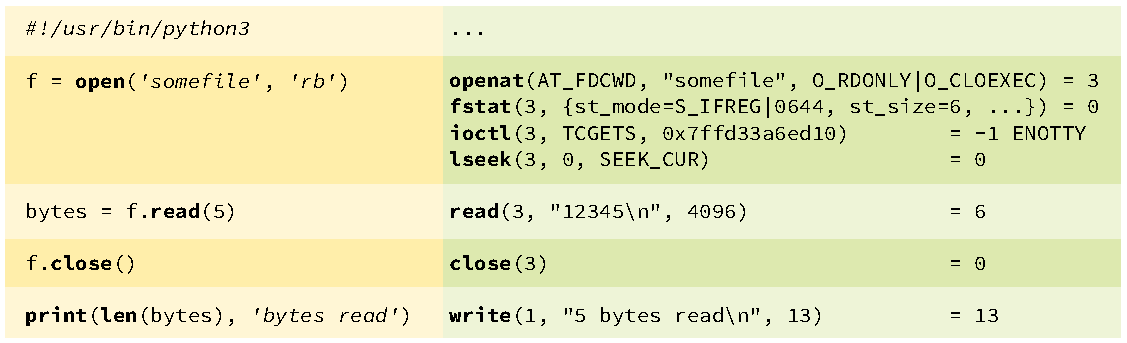
\includegraphics[scale=.8]{../images/sample-listing}
  \caption{Beispielhaftes Python-Programm (link) und dessen \strace-Ausgabe (rechts) \newline
  \emph{Anmerkung:} Die \strace-Ausgabe wurde um den relevanten Anteil gekürzt
  }
  \label{fig:sample-listing}
\end{figure*}

\section{\strace{} in Aktion}

\subsection{Analyse eines einfachen Programms}
\label{sec:simpleprogram}

Genug der Theorie. In diesem Abschnitt wollen wir uns die Ausgabe von \strace{} anhand eines
einfachen Beispiels ansehen. \autoref{fig:sample-listing} zeigt links ein kurzes Python-Skript.
Python wurde deshalb gewählt, weil es auch ohne Spezialkenntnisse leicht vertändlich ist --
deutlich einfacher als die Programmiersprache C.

Ein Shellskript ist zur Darstellung von \strace ungeeignet, da es in der Regel sehr viele externe
Programme aufruft, sog. \emph{Kindprozesse}. Gerade zu Beginn eines neu gestarteten Programmes 
werden jedoch viele Systemaufrufe durchgeführt (Laden von Bibliotheken, Übersetzungsdateien),
die für Laien erstmal schwer verständlich sind. 


Auf der rechten Seite von \autoref{fig:sample-listing} wird die unveränderte Ausgabe von \strace{}
dargestellt. Allerdings wurde nur der wesentliche Teil gelistet.

Um das Beispiel nachvollziehen zu können, starten wir das Programm folgenermaßen in einer Shell:

\begin{verbatim}
  % strace notfound.py > output.txt
\end{verbatim}

Die Ausgabeumleitung in \texttt{output.txt} wird vorgenommen damit sich die Ausgabe vom Programm
und von \strace{} nicht vermischen. Zunächst werden einige hundert Zeilen Output erzeugt die für
uns irrelevant sind. Bevor der Python-Interpreter das Programm ausführt muss erstmal der
Python-Interpreter initialisiert werden, müssen Bibliothken vom Betriebssystem geladen werden und
muss das eigentliche Skript gelesen werden. Bei einem kompilierten C-Programm\footnote{oder
natürlich auch einem Pascal- oder Go-Programm, also jeder Programmiersprache, die in ein
Maschinenprogramm übersetzt wird} wäre dieser Anteil deutlich kürzer aber dennoch relativ groß.

Die Kunst besteht darin, den eigentlichen Start des Teils des Programms zu finden, der uns
interessiert. Am besten liest man von unten nach oben. Oder man leitet die Ausgabe von \strace{}
ein eine Datei um -- wie das geht erfahren wir im nächsten Kapitel -- und sucht im Texteditor nach
einem bekannten String: Das kann eine (bekannte) Ausgabe sein oder den Namen der Datei, die
geöffnet wird.

Das Beispiel wurde so formatiert, dass die Zeilen des Programms und die korrespondierenden 
Systemaufrufe klar erkennbar sind. Dennoch nachfolgend ein paar Erklärungen.

\begin{itemize}
  \item Zunächst wird die Datei \texttt{somefile} zum Lesen geöffnet. Daraus resultiert
    ein Systemaufruf \texttt{open()}. Der Python-Interpreter verwendet das etwas modernere
    \texttt{openat()}, welches zusätzlich noch ermöglicht, anzugeben, wie relative Pfade
    behandelt werden.

    Das Ergebnis ist der \emph{Dateideskriptor} mit der Nummer 3, der bei den folgenden
    Systemaufrufen dann immer als erstes Argument angegeben wird. Dieser Dateideskriptor ist wichtig
    um die Aufrufe den verschiedenen Dateien zuordnen zu können!

    Anschließend werden Metainformationen zur Datei gelelesen, dafür wird \texttt{fstat()}
    verwendet. Zur Metainformation gehören die Größe und Zugriffsrechte der Datei. Der Aufruf
    \texttt{ioctl()} prüft, ob die Datei ein Terminal ist, \texttt{lseek()} setzt die Position
    des Lesezeigers auf den Anfang\footnote{Im Prinzip sind diese Operationen für das Programm
    gar nicht erforderlich. Das ist ein Problem der Abstraktion in der Informatik: Je "`einfacher"'
    die Programmiersprache gehalten ist, je mehr automatisch passiert, deso schwieriger wird es,
    das Verhalten des Systems auf unterster Ebene zu verstehen und deso mehr Dinge werden
    erledigt, die gar nicht erledigt werden müssten.}.

  \item Nun werden mit \texttt{f.read()} maximal 5 Bytes gelesen. Der Python-Interpreter hingegen
    puffert intern, versucht also einen ganzen Puffer von 4096 Bytes zu lesen und bekommt tatsächlich 6 Bytes. Dies ist der Rückgabewert des Systemaufrufs \texttt{read()}.

  \item \texttt{close()} gibt den Dateideskriptor 3 wieder frei.

  \item \texttt{write()} schreibt die Meldung "`5 Bytes read"' auf die Standardausgabe. Gemäß
    \autoref{tab:errno} ist der Dateideskriptor 1 die Standardausgabe.
\end{itemize}

\minisec{Fehlerfall}

Nun löschen wir die Datei \texttt{somefile,} so dass sie nicht vorhanden ist\footnote{Deshalb heißt
das Programm ja auch \texttt{notfound.py}.} und starten das Programm erneut. Die wesentliche
Zeile der \strace-Ausgabe sieht wie folgt aus:

\begin{lstlisting}
openat(AT_FDCWD, "somefile", O_RDONLY|O_CLOEXEC) = -1 ENOENT (Datei oder Verzeichnis nicht gefunden)
\end{lstlisting}

Hier ist klar erkennbar, dass die Datei nicht geöffnet wurde, weil die nicht exisistiert. Statt
einem (positiven) Dateideskriptor gibt \texttt{openat()} den Fehlercode $-1$ zurück, der gemäß
\href{http://man7.org/linux/man-pages/man3/errno.3.html}{\emph{errno(3)}} bzw. \autoref{tab:errno} 
„Datei oder Verzeichnis nicht gefunden“ bedeutet. Dieser Fehlertext ist praktischerweise in der
Ausgabe von \strace{} auch gleich mit enthalten.

Danach kommen jede Menge Fehlerausgaben, die einfach deshalb in \strace{} auftauchen, weil sich das
Python-Programm mit einer Ausnahme beendet.

\subsection{Kindprozesse und Threads}

\strace{} verfolgt standardmäßig nur den direkt gestarteten Prozess und den
Haupt-Thread\footnote{Ein \emph{Thread} (von engl. \emph{thread} = „Faden“) ist ein
Ausführungsstrang eines Programms. Mit Hilfe von Threads können Programme mehrere Dinge parallel
erledigen ohne dass damit verschiedene, komplett getrennte Prozesse gestartet werden müssen. Somit
können die Threads alle auf die gleichen Daten zugreifen.}. Aus Betriebssystemsicht (unter Linux)
sind Threads und Kindprozesse\footnote{Vereinfacht gesagt: Wenn aus einem Programm ein anderes
gestartet wird, nennt man den neu entstehenden Prozess \emph{Kindprozess.}} ziemlich ähnlich. Daher
gibt es in \strace{} auch nur eine Option: Startet man \strace{} mit der Option \texttt{-f} (für
\emph{follow),}) werden auch Kindprogramme und andere Threads beobachtet. Die Ausgabe wird jedoch
schnell undübersichtlich -- wie man etwas Abhilfe schafft beschreibt \autoref{sec:fileoutput}.

Um die Programme unterscheiden zu können beginnt jede Trace-Zeile eines Kindprozesses mit
\texttt{[pid XXXX]}, wobei \texttt{XXXX} für die jeweilige Prozess-ID steht enthält.


\subsection{Protokollierung in einer Datei}
\label{sec:fileoutput}

Wie wir in \autoref{sec:fileoutput} gesehen haben, wird die Ausgabe von \strace{} mit der des
eigentlichen Programms vermischt. Zwar schreibt \strace{} auf die Standardfehlerausgabe, jedoch
kann auch das zu beobachtenden Programm die Fehlerausgabe benutzen. Daher helfen Ausgabeumleitungen
der Shell nicht weiter. Stattdessen kann mit der Option \texttt{-o \emph{Dateiname}} die gesamte
Ausgabe von \strace{} in \texttt{\emph{Dateiname}} umgeleitet werden.

Wird beim Tracen von Kindprozessen statt \texttt{-f} die Option \texttt{-ff} angegeben, erstellt
\strace{} pro PID eine eigene Datei nach dem Schema \texttt{\emph{Dateiname}.\emph{PID}}. Das macht
das Lesen übersichtlicher. Um die Systemaufrufe auch zeitlich einordnen zu können, kann man
\strace{} mit \texttt{-t} anweisen, die aktuelle Systemzeit in die Protokolliertung hinzuzufügen,
mit \texttt{-tt} auch in der Genauigkeit von Millisekunden. Die Protokollierung von Zeitstempeln
ist unabhängig davon, ob die Ausgabe in eine Datei umgeleitet wird oder nicht.

\subsection{\strace{} einschränken}

Die vorhergehenden Abschnitte haben durch neue Optionen die Ausgabe immer noch angereichert, was
zwar nützlich ist, aber das Ganze nicht unbedingt übersichtlicher macht. In diesem Abschnitt wollen
wir den Output etwas einschränken.

Meistens interessiert man sich nicht für das Verhalten des Programms als Ganzes sondern für einen
bestimmten Teilaspekt. So könnte uns beispielsweise interessieren, warum eine Datei nicht geöffnet
werden kann. Relevant ist also eigentlich nur der \texttt{open}-Systemaufruf.

Zur Einschränkung gibt es die Option \texttt{-e trace=\emph{set}}; \texttt{\emph{set}}
steht dabei für einen oder mehrere Systemaufrufe, jeweils durch Kommata getrennt.

Nun ist es meistens eine schlechte Idee, \strace{} auf einen genauen Systemaufruf einzuschränken.
Im konkreten Beispiel (warum wird eine Datei nicht gefunden) lauern zwei Fallen: Erstens wurde
\texttt{open()} mittlerweile bei aktuellen C"=Bibliotheken durch \texttt{openat()} ersetzt, zweitens
könnte das Programm vor dem Öffnen mit \texttt{stat()} prüfen, ob die Datei überhaupt existiert.

Deshalb gibt es vordefinierte Gruppen, nämlich \texttt{\%file} für Dateioperationen.
\autoref{tab:strace_groups} liefert die wichtigsten Gruppen für Systemaufrufe.


\begin{figure*}[tb]
  \lstinputlisting[numbers=left,xleftmargin=3em,stepnumber=2]{../sample/strace_file_ls.txt}
  \caption{Einschränkung von \strace{} auf Dateioperationen}
  \label{fig:fileonly}
\end{figure*}


\begin{table}[htb]
  \centering\small
  \begin{tabular}{|lp{6cm}|}
    \hline
    \textbf{Gruppe} & \textbf{Operationen} \\
    \hline
    \texttt{\%file}          & Dateioperationen, die einen Dateinamen als Argument
                               bekommen, also beispielsweise \texttt{open,} \texttt{stat,}
                               \texttt{chmod,} \texttt{unlink,} … \\
    \texttt{\%desc}          & Dateioperationen, die einen Dateideskriptor als Argument
                               bekommen, also z.\,B. \texttt{read,} \texttt{write,}
                               \texttt{chmod,} \texttt{unlink,} … \\
    \texttt{\%process}       & Systemaurufe zur Prozessverwaltung \\
    \texttt{\%net}           & Systemaurufe zur Netzwerkprogrammierung \\
    \texttt{\%signal}        & Systemaurufe bzgl. Behandlung von Signalen \\
    \texttt{\%ipc}           & Operationen zur Interprozesskommunikation \\
    \texttt{\%memory}        & Systemaufrufe zur Speicherverwaltung \\
    \texttt{\%pure}          & Systemaufrufe ohne Argument, z.\,B. \texttt{getpid} \\
    \hline
  \end{tabular}
  \caption{Gruppen von Systemcalls für \texttt{-e trace=\emph{group}}}
  \label{tab:strace_groups}
\end{table}

Ein Beispiel: \autoref{fig:fileonly} zeigt die \emph{vollständige} Ausgabe von \texttt{strace -e 
trace=\%file ls}. Ohne diese Einschränkung wäre das Listing 66 Zeilen lang! Zunächst werden
die Biblitoheken und Übersetzungsdateien geladen, anschließend wird in Zeile 9 dann der
Dateideskriptor für das aktuelle Arbeitsverzeichnis geöffnet. Zeile 10 und 11 sind bereits
die eigentliche Ausgabe des Programms.

Es gibt noch wesentlich mehr Möglichkeiten der Filterung, die in der Manpage
\href{http://man7.org/linux/man-pages/man1/strace.1.html#OPTIONS}{\emph{strace(1)}} im Abschnitt
„Options“ und weiter unter „Filtering“ detailliert beschrieben werden.


